\documentclass[12pt]{exam}



\usepackage{graphicx}% Include figure files
\usepackage{dcolumn}% Align table columns on decimal point
\usepackage{bm}% bold math
\usepackage{latexsym}
\usepackage{amsmath,amssymb,amsthm,amsfonts}
\usepackage{subfigure}

\begin{document}
\pagestyle{head} \extraheadheight{1in}\runningheadrule
\firstpageheader{$\mbox{}$\\DATE: March 3, 2009\\PAPER NO.: - \\
DEPARTMENT $\&$ COURSE NO.: MATH 3820\\EXAMINATION: Intro. Math. Modelling}{\bf UNIVERSITY OF MANITOBA\\
$\mbox{}$
\\$\mbox{}$ \\ $\mbox{}$\\$\mbox{}$}{$\mbox{}$\\Test 1\\ PAGE NO.: \thepage\ of \numpages\\TIME: 120
minutes\\ EXAMINER: J. Arino}\runningheadrule
\runningheader{$\mbox{}$\\DATE: March 3, 2009\\PAPER NO.: - \\
DEPARTMENT $\&$ COURSE NO.: MATH 3820\\EXAMINATION: Intro. Math. Modelling}{\bf UNIVERSITY OF MANITOBA\\
$\mbox{}$
\\$\mbox{}$ \\ $\mbox{}$\\$\mbox{}$}{$\mbox{}$\\Test 1\\ PAGE NO.: \thepage\ of \numpages\\TIME: 120
minutes\\ EXAMINER: J. Arino} \vspace{-2.5cm}
\begin{center}
\begin{tabular}{cp{15.5cm}}
\hline
&\\
\end{tabular}
\end{center}
%\footer{}{Page \thepage\ of \numpages}%
%{\iflastpage{End of exam.}{Please go on to the next page\ldots}}

\addpoints

This is a 120 minutes exam, with \numquestions\; questions for a total of \numpoints\; marks. Lecture Notes are allowed.
{\sc Please show your work clearly.} A correct answer without explanation will not get full marks.
\vspace{0.1cm}

\begin{center}
\begin{tabular}{cp{15.5cm}}
\hline
&\\
\end{tabular}
\end{center}





\begin{questions}

\question[10]
The dynamics of a population of birds (measured in thousand) is described by the equation
\[
\frac{dP}{dt}=4P(1-8P^3).
\]
\begin{parts}
\part Find the equilibria.
\part Determine the local stability of each equilibrium.
\end{parts}

\vskip0.5cm
\question[10]
The population (measured in billions) of insects in generation $t$ is described as follows
$$P_{t+1}=P_t e^{4(1-3P_t)}$$
\begin{parts}
\part Find all fixed points.
\part Determine the local stability of each fixed point.
\end{parts}




\vskip0.5cm
\question[20]
Assume that an insect population, $x(t)$, is controlled by a natural predator population, $y(t)$. We make the following assumptions:
\begin{itemize}
\item In the absence of predators, the dynamics of the insects is governed by a logistic equation.
\item Preys and predators meet at a rate that is of mass action type.
\item When a contact takes place, the probability per contact that a prey dies is $k_1$. [Hint: think of mass action contact in an epidemic model.]
\item These contacts lead to an increase of the predator population with rate $k_2$.
\item The predators are subject to natural death at the per capita rate $d$.
\end{itemize}
\begin{parts}
\part Write a model describing the interaction of the 2 populations.
\part Study the model you have written: is it well-posed, what are its equilibria (and when are they realistic), can you determine the stability of these equilibria?
\part Assume that an insecticide is used to reduce the population of insects, but it is also toxic to the predators; hence, the poison kills both preys and predators at rates proportional to their respective populations. Modify your model from (a). [For bonus marks, you may want to see how this modifies the analysis you carried out in (b).]
\end{parts}



\vskip0.5cm
\question[10]
Consider the difference equation 
\[
x_{t+1}=f(x_t)
\]
with graph shown in the figure below
\begin{center}
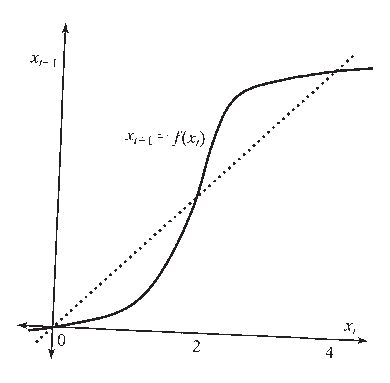
\includegraphics[width=.7\textwidth,,angle=3]{FigureTest1}
\end{center}
\begin{parts}
\part Find all fixed points. 
\part Determine the local stability of each fixed point. [Hint: what does the stability condition imply, in terms of the slope of $f$?]
\end{parts}


%\question[6]
%Show that the $2-$cycle
%$$\bar x_{1,2}=\frac{1\pm \sqrt{4r-3}}{2}$$
%of the difference equation $x_{t+1}=r-x_t^2$ is unstable if $r> 5/4$.
%\newpage



%Consider the differential equation: $\frac{dy}{dx}=y^2-4$ (Do not
%solve the equation)
%\begin{enumerate}
%\item Is the above differential equation linear or nonlinear,
%autonomous or non-autonomous? Explain.
%\item Find the equilibrium solutions.
%\item Among the 3 direction fields shown on the next page, select
%the one corresponding to the above differential equation.
%\item Use the appropriate direction field to draw an approximate
%integral curve that satisfies $y(0)=0$.
%\item  What is the behavior of your solution in part 4 as $x$ goes
%to $+\infty$; in other words what is $\lim \limits_{x\rightarrow
%\infty}y(x)$?
%\end{enumerate}
%\begin{figure}[ht]
%\centering \subfigure[]{
%\includegraphics[width=.49\textwidth]{Figure1}}
%\subfigure[]{
%\includegraphics[width=.49\textwidth]{Figure2}}
%\subfigure[]{
%\includegraphics[width=.49\textwidth]{Figure3}}
%\end{figure}



%\section*{Question 2} \marginpar{[11]}
%Consider the differential equation: $x\frac{dy}{dx}+y=x^2$
%\begin{enumerate}
%\item Find the general solution of the above differential equation.
%\item What is the interval of validity of solutions?
%\end{enumerate}


%\section*{Exercise 3}
%Consider the differential equation: $\frac{dy}{dt}=ty+t$
%\begin{enumerate}
%\item Show that $y=-1$ is a solution of the above differential equation.
%\item Find the general solution of the above differential equation.
%\end{enumerate}

%\section*{Question 3}\marginpar{[14]}
%Consider the differential equation:
%$\frac{dy}{dx}=-\frac{1}{2}xy^3(1+x^2)^{-1/2}$
%\begin{enumerate}
%\item Show that $y(x)=0$ is a solution of the above differential equation.
%\item Find the general solution of the above differential equation.
%\item Find the solution that satisfies $y(0)=1$.
%\end{enumerate}

%\newpage
%\section*{Question 4}\marginpar{[11]}
%A population of butterflies in a forest increases at a rate $r$
%proportional to the total population. Initially, there are $20,000$
%butterflies, and birds eat $1,000$ butterflies per days.
%\begin{enumerate}
%\item Construct a mathematical model (\emph{i.e.}, differential equation and initial condition) to determine the population of
%butterflies in the forest at any time. Explain your variables,
%parameters and the units used. (Do not solve the equation)
%\item In the
%absence of predators (\emph{i.e.}, with no birds), biologists
%observe that the population triples each week. Calculate the rate of
%birth $r$ of butterflies in the forest (leave your answer with
%logarithms).
%\end{enumerate}




\end{questions}
\end{document}
